\documentclass{ltjsbook}
\usepackage{docmute} 
\usepackage{../myStyle} 

\begin{document}
\VerbatimFootnotes
\chapter{記号の入力とキーボードの場所}
\label{signs}
プログラミングのミスでよくあるのが打ち間違い，スペルミスです。Xとx，Sとsなど大文字と小文字で形が同じものや，l(エルの小文字)と1(数字のイチ)の違いなどは，プログラミング用フォントにして違いがわかるようにするとか，文字列の意味から類推する(Normalとあればノーマルであって，ノーマ・イチではないと察する)など工夫が必要かもしれません。

また，理由はよくわからないのですが頻発するスペルミスは，データ(data)をデート(date)と書いてしまうことです。データはラテン語のdatum(与えられたもの)の複数形なのですが，最近のデータサイエンスの文脈ではdataも単数形と考えるようです。ともかく，日付を表すdateとは由来も意味もスペルも全て違うので，気をつけましょう。

さて，これらはまだ序の口。プログラミングのコードを読んでも，日本語の五十音に入っていない記号の違いがわからない，どこでそれが入力できるかわからない，質問しようにも読み方がわからないといったものもあります。ここではこれらをまとめて解説します。記号の上では微妙な違いですが，当然形が違うのでプログラミング上は違う文字として扱われますので，形の細部までよくみてください。なお，プログラミングでつ変わる時は言語に依存することもありますので，ご注意ください\footnote{たとえばコメントアウトはC言語では\verb|\\|，Rでは\verb|#|，TeXでは\verb|%|など，それぞれ異なります。}。

特に目立つのはハイフンとチルダ，アンダースコアの入力ミスです。それぞれ文字を書く領域における位置が違ったり，形が違ったりするのでよくみてください。
\begin{center}

	\Large{
		\begin{tabular}{ll}
			ハイフンは真ん中  & \verb|A-B| \\
			アンダースコアは下 & \verb|A_B| \\
			オーバーバーは上  & \verb|A¯B| \\
			チルダはニョロ   & \verb|A~B| \\
		\end{tabular}
	}

\end{center}

これを踏まえて，そのほかの記号の名称や意味を表\ref{keyboardName}で確認しましょう。
\begin{table}[ht]
	\centering
	\caption{記号と読み方}
	\label{keyboardName}
	\begin{tabular}{ccl}
		記号        & 読み方            & 解説                                                                         \\\hline
		:         & コロン            & 英文中では「すなわち」などの意味。セミコロンと間違えないように                                            \\
		;         & セミコロン          & 英文中では文章の区切り，接続詞のようにつかう                                                     \\
		.         & ピリオド           & 英文の終わりを意味する。日本語で言う句点                                                       \\
		,         & カンマ            & 英文の区切りを意味する。日本語で言う読点                                                       \\
		\verb|@|  & アットマーク         & メールアドレスに用いられることで有名                                                         \\
		\verb|$|  & ドルマーク          & 米国の通貨単位。Rでは変数名指定のときにもちいる                                                   \\
		/         & スラッシュ          & 割り算の記号                                                                     \\
		*         & アスタリスク         & 掛け算の記号                                                                     \\
		+         & プラス            & 足し算の記号                                                                     \\
		-         & マイナス           & 引き算の記号                                                                     \\
		\verb|^|  & ハット            & 累乗の計算の記号                                                                   \\
		=         & イコール           & 等号。プログラミングでは\verb|==|で一致しているかどうかの判定にも                                      \\
		!         & エクスクラメーション     & 強調。プログラミングでは否定(NOT)の意味になることも                                               \\
		\verb|_|  & アンダースコア，アンダーバー & \begin{tabular}{l}位置に注意。ハイフンではなく文字領域の下の線 \\
			                                                   変数名をつなげる時(ex. \verb|snake_case|)に使ったりする\end{tabular} \\
		\verb|~|  & チルダ            & \begin{tabular}{l}Rでは独立変数と従属変数をつなぐときに使う \\
			                                                   ハイフンやオーバーライン，アンダースコアと間違えられる率高め\end{tabular}          \\
		\verb|¯|  & オーバーライン，オーバーバー & アンダースコアの逆。滅多に使わないが。文字化けを直したときにみられる。                                        \\
		\verb|%|  & パーセント          & プログラミングではコメントアウトの時などに使われたりする                                               \\
		\verb|&|  & アンパサンド         & プログラミングにおけるAND(論理積)の記号など                                                   \\
		\verb|||  & 縦棒             & プログラミングにおけるOR(論理和)，条件付き確率の記号にも                                             \\
		\verb|\|  & バックスラッシュ       & プログラミングではコメントアウトの時などに使われたりする                                               \\
		\verb|"|  & ダブルクォーテーション    & 文字列の開始・終了を表す。同じ記号で閉じる                                                      \\
		\verb|'|  & シングルクォーテーション   & 文字列の開始・終了を表す。同じ記号で閉じる                                                      \\
		\verb|`|  & バッククォーテーション    & 文字列の開始・終了を表す。同じ記号で閉じる                                                      \\
		\verb|[]| & 大括弧            & プログラミングでは配列を意味することがある                                                      \\
		\verb|{}| & 中括弧            & プログラミングではブロックの開始と終了を意味することがある                                              \\
		\verb|()| & 小括弧            & 数式のまとまりを表す                                                                 \\\hline
	\end{tabular}
\end{table}


一般的な日本語キー配列の場合，1つのキーに4つの文字・記号が割り当てられていますが，英語入力モードの場合はキーの左側，日本語入力モードはキーの右側を見ることになります。キーを押すと下の段の文字が入力されますが，シフトキーを押しながらキーを押すことで上の段の文字が入力されることになります(図\ref{JPkeyChange})。

これを踏まえて，日本語キーについては\ref{jpKeyAssign}，USキーについては図\ref{usKeyAssign}に代表的な記号とキー配列の位置を示しました。入力に困った場合は一度図を見て確認してください\footnote{USキー配列はキートップに一種類の文字しかなく，美しい配置なのでおすすめです。}。
\begin{figure}[ht]
	\centering
	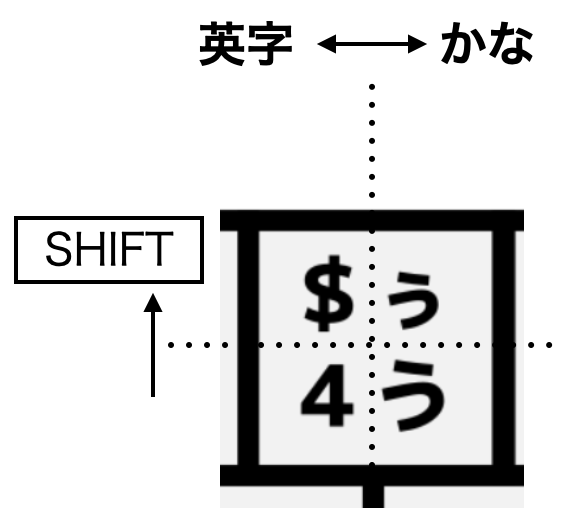
\includegraphics[keepaspectratio,width=4cm]{../common_contents/figures/JapaneseKeyChange.png}
	\caption{日本語キーで入力する場合}
	\label{JPkeyChange}
\end{figure}
\begin{figure}[ht]
	\centering
	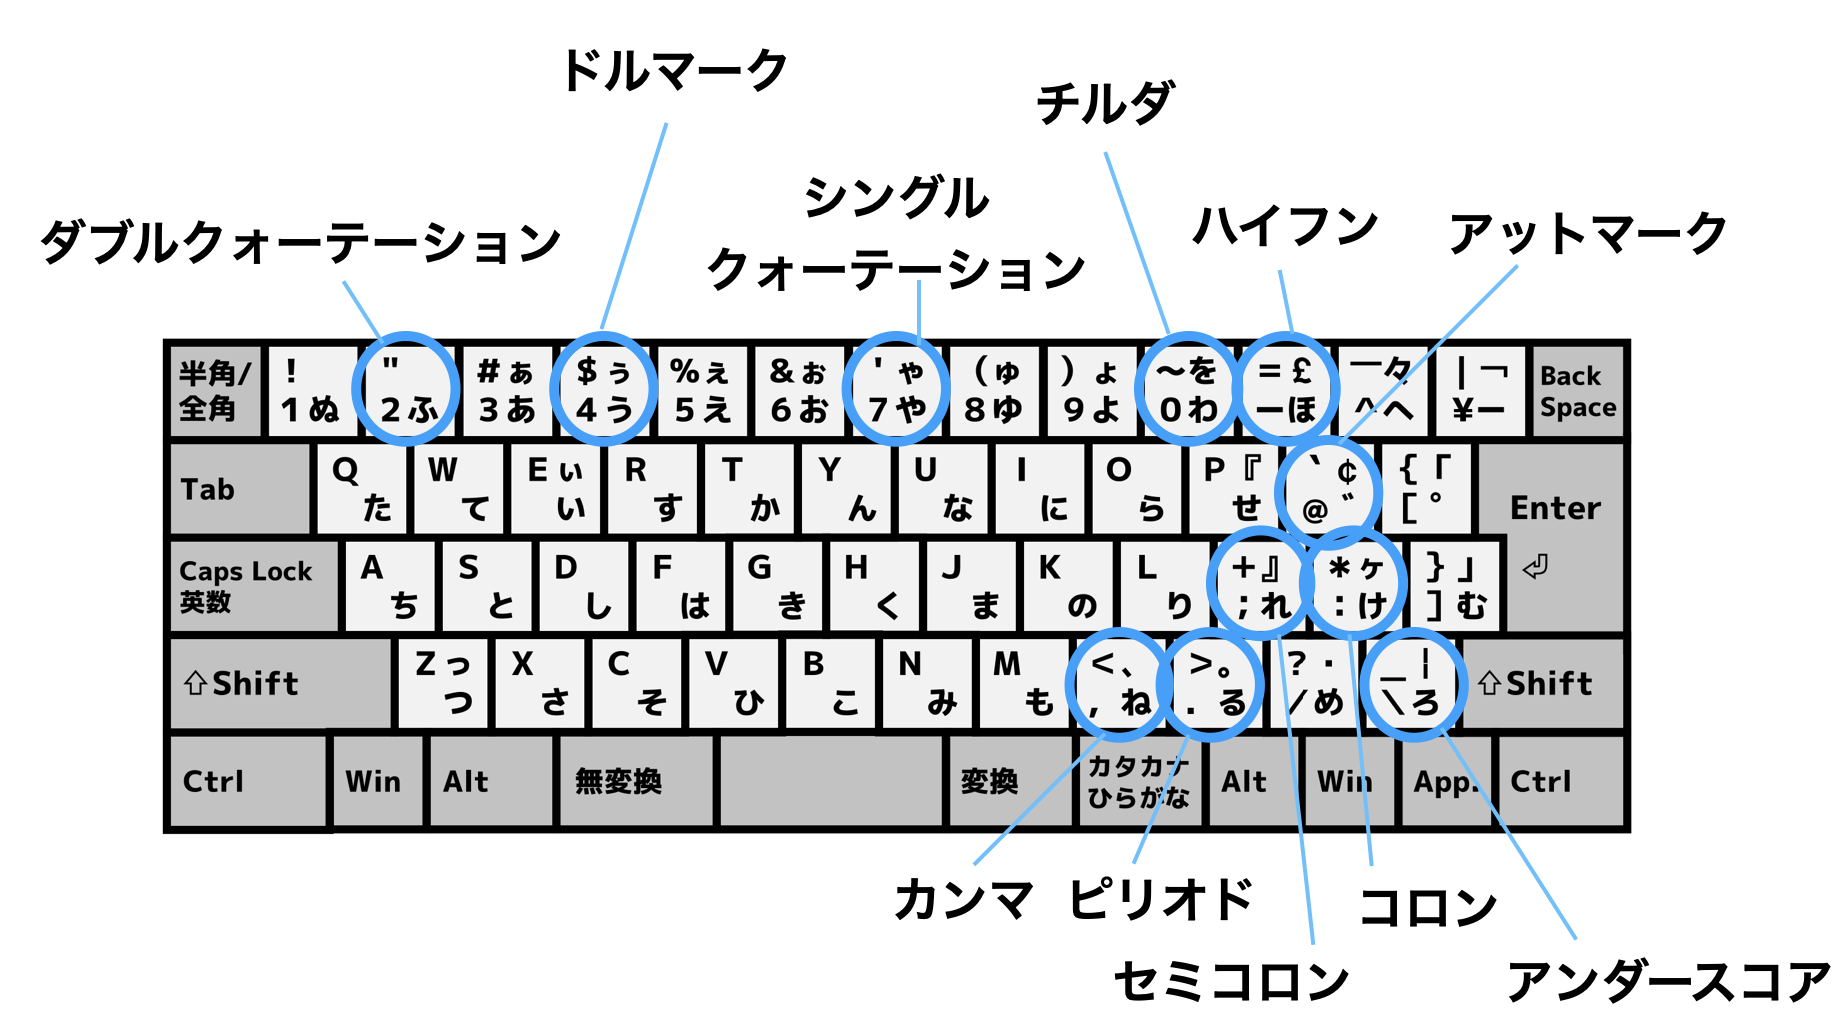
\includegraphics[keepaspectratio,width=0.8\linewidth]{../common_contents/figures/JPkeyAssign.png}
	\caption{代表的な記号と日本語キー配列}
	\label{jpKeyAssign}
\end{figure}
\begin{figure}[ht]
	\centering
	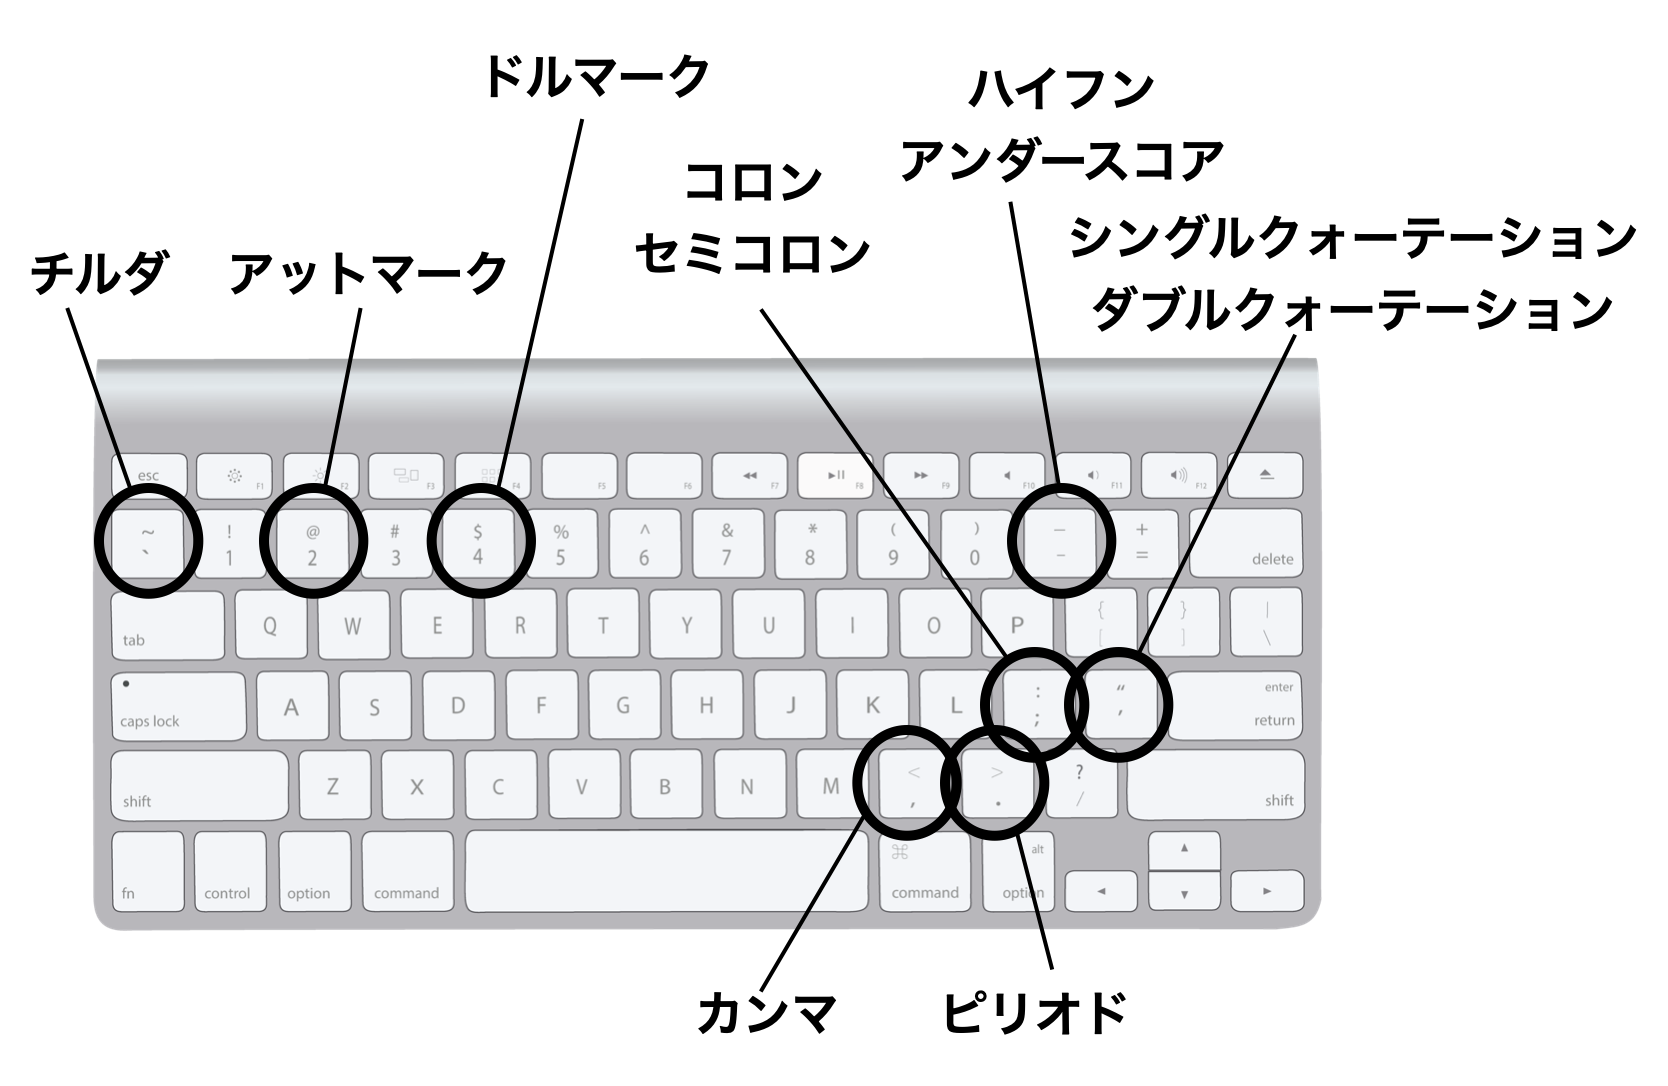
\includegraphics[keepaspectratio,width=0.8\linewidth]{../common_contents/figures/usKeyAssign.png}
	\caption{代表的な記号とUSキー配列}
	\label{usKeyAssign}
\end{figure}

\end{document}